\chapter{Mathematically Conditioning}

\section{Introduction}

\subsection{Problem Statement}

Suppose we want to compute \( f(x) \) at \( x = \bar{x} \). Suppose we do not know \( \bar{x} \) exactly, but only an approximation of it, \( \hat{x} \) to \( \bar{x} \) where \( \hat{x} \doteq \bar{x} \).

\begin{definition}[Signed Relative Error]\index{Signed Relative Error}
    The \term{signed relative error} in approximation of \( \bar{x} \) by \( \hat{x} \) is defined as \[
        \delta x = \frac{\hat{x} - \bar{x}}{\bar{x}}.
    \]
\end{definition}

We want to compute \( f(\bar{x}) \), but what we get is \( f(\hat{x}) \) -- a slightly different problem. \begin{align*}
    f(\hat{x})
     & = f(\bar{x}(1 + \delta x))                                                      \\
     & = f(\bar{x} + \bar{x} \delta x)                                                 \\
     & = f(\bar{x}) + (\bar{x} \delta x) f'(\bar{x}) + \dots
     & \text{Taylor series expansion}                                                  \\
     & \doteq f(\bar{x}) + (\bar{x} \delta x) f'(\bar{x})                              \\
     & = f(\bar{x}) \left( 1 + \frac{\bar{x} f'(\bar{x})}{f(\bar{x})} \delta x \right)
\end{align*}

The relative error in approximating \( f(\bar{x}) \) by \( f(\hat{x}) \) is \[
    \frac{|f(\hat{x}) - f(\bar{x})|}{|f(\bar{x})|} = \left| \frac{\bar{x} f'(\bar{x})}{f(\bar{x})} \right| | \delta x |.
\]

An accurate estimation is when \( \left| \frac{\bar{x} f'(\bar{x})}{f(\bar{x})} \right| \) is small. This is known as the \term{condition number} of the problem.

\begin{definition}[Condition Number]\index{Condition Number}
    The condition number of evaluating \( f(x) \) is defined as \[
        \kappa_f(x) = \left| \frac{x f'(x)}{f(x)} \right|.
    \]
\end{definition}

\begin{remark}
    Note we nave not written any algorithm. The condition number is a pure mathematical concept.
\end{remark}

\begin{remark}
    When \( \kappa_f(x) \) is small, the problem is \term{well-conditioned}\index{Well-Conditioned Problem}. When \( \kappa_f(x) \) is large, the problem is \term{ill-conditioned}\index{Ill-Conditioned Problem}.
\end{remark}

\begin{remark}[Rule of Thumb]
    You loose approximately \[
        \log_2 \kappa_f(x)
    \] bits of accuracy when you approximate \( f(\bar{x}) \) by \( f(\hat{x}) \).
\end{remark}

\begin{example}
    Consider \( f(x) = \sqrt{x} \). Let \( \hat{x} \doteq \bar{{x}} \).

    How well does \( f(\hat{x}) \) approximate \( f(\bar{x}) \)?

    Let's look at the conditional number for this function, \begin{align*}
        \kappa_{\sqrt{\null}}(x)
         & = \left| \frac{x \frac{d}{dx} \sqrt{x}}{\sqrt{x}} \right|                      \\
         & = \left| \frac{x \cdot \frac{1}{2} \cdot \frac{1}{\sqrt{x}}}{\sqrt{x}} \right| \\
         & = \frac{1}{2}.
    \end{align*}

    Since \( \kappa_{\sqrt{\null}}(x) < 1 \), \( \sqrt{\hat{x}} \) is a good approximation to \( \sqrt{\bar{x}} \). Any error \( \delta x \) in \( \hat{x} \) becomes \( \frac{1}{2} \delta x \) in \( f(\hat{x}) \) in the relative sense.

    We draw the conclusion that evaluating square roots is a well-conditioned problem. If we have an numerically stable algorithm to compute square roots, we should get an accurate result.
\end{example}

\begin{remark}
    If we use a numerically stable algorithm on a well-conditioned problem, we should get an accurate result.

        {~~~}

    The contra positive is also true: if we get an inaccurate result, then either the problem is ill-conditioned or the algorithm is not numerically stable.
\end{remark}

\begin{example}
    Consider \( f(x) = \ln(x) \). Let \( \hat{x} \doteq \bar{x} \).

    Suppose we want to evaluate \( \ln(0.999) \), where \( 0.999 \) is an intermediate result with some error. We will get \( \ln(0.999) \doteq -1.0005 \times 10^{-3} \).

    Consider a \( 0.01\% \) relative change to argument, \[
        \ln(0.999(1+0.00001)) = -9.0049 \times 10^{-4} = -1.0005 \times 10^{-3} (1 + 0.09996)
    \] We see that the relative error in the result is \( 9.996\% \). A small change in the argument results in a large change in the result. This tells us that evaluating logarithms must be an ill-conditioned problem.

    \begin{align*}
        \kappa_{\ln}(x) & = \left| \frac{x \frac{d}{dx} \ln(x)}{\ln(x)} \right| \\
                        & = \left| \frac{x \frac{1}{x}}{\ln(x)} \right|         \\
                        & = \frac{1}{\ln(x)}.
    \end{align*}

    At \( x = 0.999 \), we have \[
        \kappa_{\ln}(0.999) = \frac{1}{\ln(0.999)} \doteq 999.5.
    \]

    For \( x \) near \( 0.999 \), the effect of a small error is magnified by approximately 1000.
\end{example}

\begin{example}
    Is \( f(x) = \ln(x) \) always ill-conditioned? No.

    \begin{figure}[H]
        \centering
        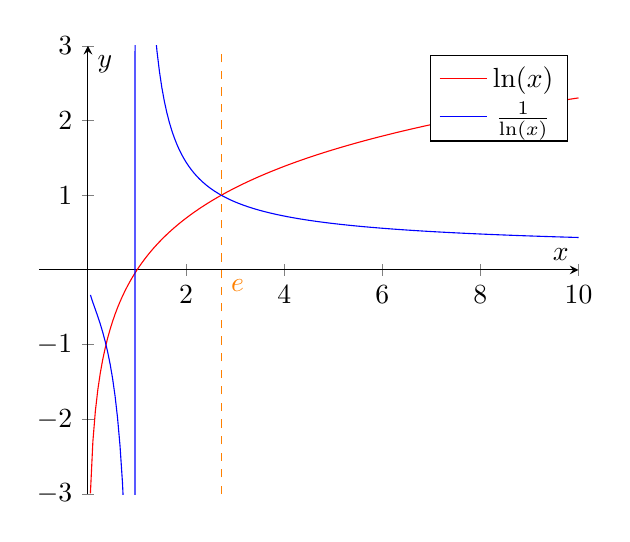
\begin{tikzpicture}
            \begin{axis}[
                    axis lines = middle,
                    xlabel = \( x \),
                    ylabel = \( y \),
                    xmin = -1,
                    xmax = 10,
                    ymin = -3,
                    ymax = 3,
                    ytick = {-3, -2, -1, 0, 1, 2, 3},
                ]
                % ln(x)
                \addplot [
                    domain=0:10,
                    samples=200,
                    color=red,
                ] {ln(x)};
                \addlegendentry{\( \ln(x) \)}
                % 1/ln(x)
                \addplot [
                    domain=0:10,
                    samples=200,
                    color=blue,
                ] {1/ln(x)};
                \addlegendentry{\( \frac{1}{\ln(x)} \)}

                \draw [orange,dashed] (axis cs:2.718281828459045, -3) -- (axis cs:2.718281828459045, 3);
                \node [orange,below right] at (axis cs:2.718281828459045, 0) {\( e \)};
            \end{axis}
        \end{tikzpicture}
    \end{figure}

    We see that \( \kappa_{\ln}(x) \) is small for \( x \) near \( 0 \) and \( x > e \).

    What about \( x \) near \( 1 \)? We introduce a new argument \( w \), \[
        \ln(x) = \ln(1 + w)
    \]

    Consider \( g(w) = \ln(1 + w) \).
    \begin{align*}
        \kappa_{g}(w)
         & = \left| \frac{w \frac{d}{dw} \ln(1 + w)}{\ln(1 + w)} \right|
        \\
         & = \left| \frac{w \cdot \frac{1}{1 + w}}{\ln(1 + w)} \right|
    \end{align*}

    We know that \( f(x) \) is ill-conditioned for \( x \to 1, w \to 0 \). What is \( \kappa_{g}(w) \) for \( w \to 0 \)?

    Using L'H\^opital's Rule, \[
        \lim_{w \to 0} \left| \frac{w \cdot \frac{1}{1 + w}}{\ln(1 + w)} \right| = 1.
    \]

    \begin{figure}[H]
        \centering
        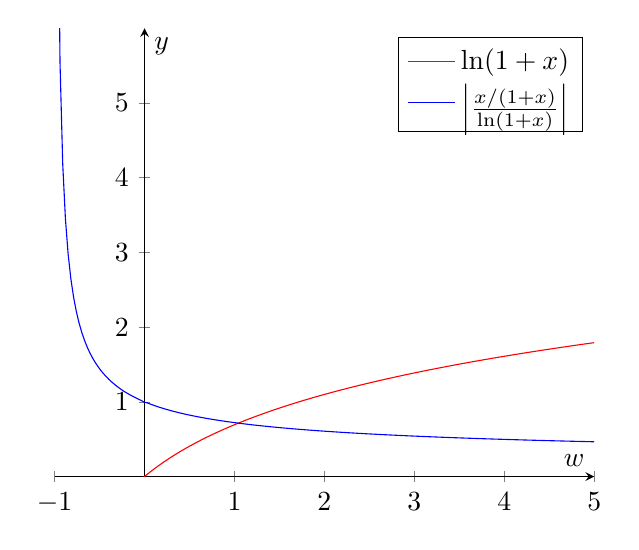
\begin{tikzpicture}
            % Plot ln(1+x) in red, |(x/(1+x))/ln(1+x)| in blue
            \begin{axis}[
                    axis lines = middle,
                    xlabel = \( w \),
                    ylabel = \( y \),
                    xmin = -1,
                    xmax = 5,
                    ymin = 0,
                    ymax = 6,
                    ytick = {0, 1, 2, 3, 4, 5},
                ]
                % ln(1+x)
                \addplot [
                    domain=-1:5,
                    samples=200,
                    color=red,
                ] {ln(1+x)};
                \addlegendentry{\( \ln(1 + x) \)}
                % |(x/(1+x))/ln(1+x)|
                \addplot [
                    domain=-1:5,
                    samples=200,
                    color=blue,
                ] {abs((x/(1+x))/ln(1+x))};
                \addlegendentry{\( \left| \frac{x/(1+x)}{\ln(1 + x)} \right| \)}
            \end{axis}
        \end{tikzpicture}
    \end{figure}
\end{example}

\begin{remark}
    In \texttt{libm}, the C standard math library, the function \texttt{log1p} is used to compute \( \ln(1 + x) \) for small \( x \). This function is numerically stable for small \( x \).
\end{remark}

\begin{example}
    How to accurately evaluate \[
        f(x) = x = \sqrt{x^2 - 1} \qquad \text{for } |x| > 1
    \]
\end{example}

% TODO: Lecture 10 - 2025-01-27